\chapter{Testing and deployment}

\section{Containerised deployment}
It's common practice to package dependencies and runtimes along with an app, to ensure consistency in how it runs on different operating systems and environments, with Docker being the most popular option. A Docker container is lightweight, portable and can function on its own. Its structure is described using a Dockerfile, placed in a project's root folder; the process is usually based on a pre-existing image, such as the minimalistic Alpine Linux, only 5 megabytes in size. Contained instructions are executed in order, and the resulting image can then be run on any machine with Docker installed. The program is isolated from the host when run in this way, but can access specified resources near-natively.

I packaged the server project for distribution with Docker. I used the gradle:8.11.1-jdk21 image for the build stage of the app. The code is copied into the container, then built using Gradle. The runtime stage then uses openjdk:21-slim (based on Debian 12 Bookworm), copies the compiled \verb|.jar| file and runs it. Networking and persistent storage could be added as command line options, but I instead used Docker Compose, a tool that allows the declaration of layered apps, made up of services provided by containers. As well as exposing the server's default port, a volume is added that covers the app's root folder. This means the database file stays on the disk between runs, but rebuilding the container still deletes it as expected. The volume could also be bound to a folder on the host, making the database file readily inspectable and modifiable without entering the container.

\section{Performance testing}

As the app's communication does not follow typical REST patterns, and the correctness of the created map is best checked visually, I tested the app's runtime performance and scalability.
Machine 1 is a Windows 11 desktop computer with an AMD Ryzen 5 7600X processor, 32GB of RAM and an AMD Radeon RX 6750 XT GPU. It has a stable 1Gbps Ethernet connection. Machine 2 is a laptop running Arch Linux with an AMD Ryzen 5 7520U CPU, 16GB of memory, and integrated AMD Radeon graphics. During the tests, the laptop used 5GHz Wi-Fi with a measured speed of 84.5/171 Mbps (download/upload). In all instances, the program was started using Gradle and Oracle OpenJDK version 21.0.5 (instead of JDK version 23, to ensure compatibility). 

I performed load time tests using two PBF files: the cities of Budapest (39,3 MB) and Szeged (6 MB), taken from BBBike. \verb|Load only| means the server was already running and the client requested all data from the database -- the time displayed is in real-time seconds (not processor time) and is counted from pressing the \verb|Load server| button to the point the \verb|Loading| banner message disappears. \verb|Rebuild| also adds file upload and database build times, the duration is calculated from pressing \verb|Open| in the file upload dialog to the \verb|Loading| banner disappearing. The client was ran on machine 1, with the server project containerised on either of the machines. The graphics capabilities of machine 2 proved insufficient for the Budapest scene to be rendered consistently, so it was not used as a client during the tests.

\begin{center}
    \begin{tabular}{l|cc|cc}
        \multicolumn{1}{c}{} & \multicolumn{2}{c}{Budapest} & \multicolumn{2}{c}{Szeged} \\
        \hline
        Server & LO & R & LO & R \\
        \hline
        Machine 1 & 17.86s & 46.18s & 6.67s & 9.29s \\
        Machine 2 & 39.91s & 52.31s & 2.18s & 5.02s \\
    \end{tabular}
\end{center}
It's clear that the main bottleneck on performance is the amount of raw data contained in the processed file. Since Budapest has around 400,000 buildings and the Szeged chunk consists of less than 20,000, loading times scale slower than an expected linear function would. The base performance is mostly impacted by database access in the initialisation step. PBF file transfer to the host increased runtime by about 1.5--2$\times$. The difference between load only and rebuild times has a roughly linear correlation to the source file size.
The outlying value of 46.18 seconds is due to the overuse of just one physical disk. Even though network transfers generally slow things down, the Szeged test results highlight the advantage of separating the two projects as more processing power could be utilised overall. In Budapest's case, the slower transfer rates removed this advantage; an adequately equipped server would likely make the app faster in such a distributed configuration when compared to a single consumer-grade machine.

\begin{figure}[!h]
    \centering
    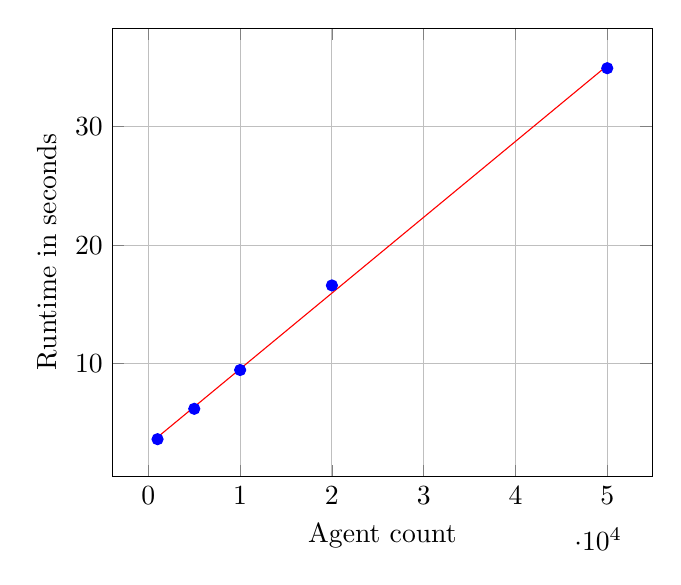
\begin{tikzpicture}
    \begin{axis}[
        xlabel={Agent count},
        ylabel={Runtime in seconds},
        xmode=linear,
        grid=major
    ]
    
    \addplot[
        color=blue,
        mark=*,
        only marks
    ] coordinates {
        (1000, 3.64)
        (5000, 6.20)
        (10000, 9.47)
        (20000, 16.6)
        (50000, 34.91)
    };
    
    \addplot[
        color=red,
        domain=1000:50000,
        samples=100,
        smooth
    ] {0.0006392139 * x + 3.169522};
    
    \end{axis}
    \end{tikzpicture}
    \caption{Plot of simulation scalability}
\end{figure}

\label{perftesting-heatmap}
I also tested the time complexity of the simulation. For this, a scenario was run on the Budapest dataset with time constraints of 08:00--09:00, and agent counts of 1000, 5000, 10000, 20000 and 50000. This test was conducted on machine 1 entirely. As expected, the increase in runtime is almost exactly linear. A comparison of the resulting heatmaps can be seen in the appendix, at~\ref{comparison_heatmap}. Based on this, it's generally useful to add at least 20000 agents for a more statistically significant result.

Finally, I evaluated the space usage of the client and server using the Budapest and Szeged datasets. The result shows that even for an entire city's worth of unique models and tag data, the used RAM is not more than what typical consumer-grade machines have. On the server side, using a database as a primary storage solution is vindicated as the overall storage requirement is acceptable and the app's memory usage hovers around a gigabyte constantly, aside from a few burst increases when reading and sending data.

\begin{center}
    \begin{tabular}{l|cc|cc}
        \multicolumn{1}{c}{} & \multicolumn{1}{c}{Budapest} & \multicolumn{1}{c}{Szeged} \\
        \hline
        Frontend (RAM) & 5070 MB & 748 MB \\
        Backend (DB size) & 622 MB & 77.9 MB \\
        \end{tabular}
\end{center}

Before finishing the project, I often tried to specifically cause errors while using it, a form of negative testing. This may sound simple, but was critical in finding bad user interface decisions that could be patched to reduce errors. Using conventional testing methods, I likely would've had difficulty fixing these issues. For example, I discovered:\begin{itemize}
    \item The UI not responding to resizing the window, buttons would simply go out of bounds
    \item Parallel queries from a single client causing completely random display behaviour
    \item Buildings still being clickable while popups were open, causing the interface to be unusable
    \item The server overloading the client with responses, causing missed data, or even crashes
\end{itemize}